\documentclass[a4paper]{article}

\usepackage[utf8]{inputenc}
\usepackage[T1]{fontenc}
\usepackage{textcomp}
\usepackage{listings}
\usepackage{lmodern}
\usepackage{amsfonts}
\usepackage{titling}
\usepackage{lipsum}
\usepackage[left=1in, right=1in, bottom=1in, top=1in]{geometry}
\usepackage{mathtools}
\usepackage{amsthm}
\usepackage{tcolorbox}
\usepackage{hyperref}
\usepackage{xcolor}
\usepackage{graphicx}
\usepackage{makeidx}
\usepackage{tikz}
\usepackage{cases}
\usepackage{apacite}
\usepackage{tkz-berge}
\usepackage{lastpage}
\usepackage{fancyhdr}
\pagestyle{fancy} 
\usepackage{url}
\usepackage{tgtermes}
\usepackage{algorithm2e}
\usepackage{sectsty}
\usepackage{subcaption}
\usepackage{setspace}
\usepackage{float}
\usepackage{amsmath, amssymb}
\rhead{Page~\thepage~of~\pageref{LastPage}.}
\cfoot{}

% figure support
\usepackage{import}
\usepackage{xifthen}
\pdfminorversion=7
\usepackage{pdfpages}
\usepackage{transparent}
\newcommand{\incfig}[2][1]{%
    \def\svgwidth{#1\columnwidth}
    \import{./figures/}{#2.pdf_tex}
}
\definecolor{darkgreen}{rgb}{0.0, 0.5, 0.0}
\lstset{
tabsize = 4, %% set tab space width
showstringspaces = false, %% prevent space marking in strings, string is defined as the text that is generally printed directly to the console
numbers = left, %% display line numbers on the left
commentstyle = \color{darkgreen}, %% set comment color
keywordstyle = \color{blue}, %% set keyword color
stringstyle = \color{red}, %% set string color
rulecolor = \color{black}, %% set frame color to avoid being affected by text color
basicstyle = \small \ttfamily , %% set listing font and size
breaklines = true, %% enable line breaking
numberstyle = \tiny,
  frame=none,
  xleftmargin=2pt,
  stepnumber=1,
  belowcaptionskip=\bigskipamount,
  captionpos=b,
  escapeinside={*'}{'*},
  language=haskell,
  tabsize=2,
  emphstyle={\bf},
  showspaces=false,
  columns=flexible,
  showstringspaces=false,
  morecomment=[l]\%,
}

%mathstyling
\theoremstyle{plain}
\newtheorem{thm}{Theorem}[section]
\newtheorem{lem}[thm]{Lemma}
\newtheorem{prop}[thm]{Proposition}
\newtheorem*{cor}{Corollary}

\theoremstyle{definition}
\newtheorem{defn}{Definition}[section]
\newtheorem{conj}{Conjecture}[section]
\newtheorem{exmp}{Example}[section]
\newtheorem{axiom}{Axiom}
\theoremstyle{remark}
\newtheorem*{rem}{Remark}
\newtheorem*{note}{Note}

\pdfsuppresswarningpagegroup=1

\begin{document}
	\begin{titlepage}
	\begin{center}
	\large
	University of Warwick \\
	Department of Computer Science \\
	\huge
	\vspace{50mm}
	\rule{\linewidth}{0.5pt} \\
	CS132: Computer Organisaton \& Architecture \\
	\vspace{5mm}
	\Large
	Coursework 2
	\rule{\linewidth}{0.5pt}
	\vspace{5mm}
	\begin{figure}[H]
	\centering
	
\includegraphics[width=0.4\textwidth]{crest_black.eps}
	\end{figure}
	\vspace{33mm}
	2108182\\
	\today
	\end{center}
	\end{titlepage}
\tableofcontents
\newpage
\section{Introduction}
\subsection{Problem 1}

\subsection{Problem 2}
\section{Problem 1}
\subsection{Power set}
The first problem of coursework $2$ introduces the implementation of a "Power set" in code. However, in order for this code to be written, it is first important to break down as to what requires to actually be defined.
\begin{tcolorbox}[colback=black!3!white,colframe=black!60!white,title=\begin{defn}Power Set \label{Power Set}\end{defn}]
The power set of a finite set $S$, denoted as $2^{S}$, is the set that contains all subsets of $S$ as its elements. Formally, 
\begin{align*}
	2^{S} = \{ X : X \subseteq S \}
\end{align*}
The cardinality of the set (number of elements denoted as $|S|$), is then, as a corollary:
\begin{align*}
	|2^{S}|&=2^{|S|} \\
	       &=\sum_{i=0}^{|S|} {}^{|S|}C_k
\end{align*}
Note that for the sake of this paper, we will not be discussing if $S$ is infinite, as the code will be implemented with the assumption that the input is also finite.
\end{tcolorbox}
\begin{flushleft}
And the intuition behind this corollary is important for our implementation, as it in fact gives us a big hint as to how Problem $1$ could be implemented as code. Consider the sets $S = \{x,y\}$, $S' = \{ x,y,z \}$, $2^{S}$ and $2^{S'}$. In terms of decision trees for their power sets, it would be visualised as the following:
\end{flushleft}
\begin{figure}[H]
    \centering
    \incfig[0.8]{2s}
    \caption{Visualisation of the power set $2^{S}$}
    \label{fig:2s}
\end{figure}
\begin{figure}[H]
    \centering
    \incfig[0.9]{2sprime}
    \caption{Visualisation of the power set $2^{S'}$}
    \label{fig:2sprime}
\end{figure}
\begin{flushleft}
These figures make it apparent as to how the cardinality $|2^{S}| = 2^{|S|}$ precisely works. That is, for each new element to the set $S$, we must add a new branch of yes or no decisions for all previously existing power set elements. When the answer is no to the new element for all branches, we get $2^{S}$. With all answers yes, we obtain $x \in 2^{S} : x \cup z$. \\

Formally, let us define $S' = S \cup \{ \zeta \}$ where $\zeta$ is the new arbitrary element of a finite set $S$. Then, we can obtain the following formula for their power set:
\end{flushleft}
\begin{align*}
	2^{S^{*}} &= \{ x \in 2^S : x \cup \{ \zeta \}\}\\
	2^{S'} &= 2^S \cup 2^{S^{*}}
\end{align*}
\subsection{Pseudocode}
Now that the intuition and the mathematical formula has been well defined, we could write the pseudo code that we will implement into C. This will help us plan the structure of what is to come when writing our code.\\

\begin{algorithm}[H]
	\caption{Power set pseudocode}
	\KwData{User input of elements into our set $S$ }
	\KwResult{A printed $2^{S}$ }

	Begin \\
	Take input from user\;
	Initialise output variable array\;
	\While{Our counter is not at the size of $|S| + 1$ elements}{
		Initialise counter $ = 1$\;
		\eIf{first element}{Add first singleton set to output variable\;}{Add new element to each existing set in output variable and store them in output variable\;}
		counter $=$ counter$+1$\;
	}
	Add empty set to output variable\;
	Print output variable\;
	End
\end{algorithm}

\begin{flushleft}
Now that the pseudocode has been defined, we could move onto the written code and explaining each line's design.
\end{flushleft}
\subsection{Explanation of code design}
This section will require that the file $powerset.c$ is opened as the lines of code that are expressed in this section correspond to the lines of code of that file.
\begin{itemize}
	\item (Lines $8-16$) The definition of a two power was defined to keep the numbers in unsigned integers. This helps reduce code as type casting is not required as the original package assumes the output not to be an integer
	\item (Lines $36-40$) arraySize is converted into integer during the actual method to ensure that the user does not go over and including the number $20$. 
	\item (Lines $52-55$) The sizes of the variables are as following:
		\begin{itemize}
			\item S as input arraySize as this is the amount of elements it holds.
			\item powerSetS as $2^{arraySize}$ as this is the theoretical amount of elements.
			\item powerSetSStar as $\text{arraySize}-1$ because it will only require at maximum have the same amount of elements that exist in $S$ at that time. However, we subtract another $-1$ because we add the empty set separate for our algorithm.
			\item Memory size as $100$ as this is a good amount to assume that the string will not be longer than $99$ characters.
		\end{itemize}
	\item (Lines $104-107$) It was decided that all subsets will be listed in new lines because otherwise it would be a very long singular line and even difficult to read.
\end{itemize}
Assumptions include that the set is finite and is not larger or including cardinality size $20$. The reason for this is because the stack in the CPU is limited to $8mb$. Increasing this value would not necessarily help much, given that the size set grows exponentially. Re-assigning non-default amount to stack by increasing it is also not necessarily better, as it can lead to stack overflow. Furthermore, unsigned int was used as the general type for numbers as we cannot have negative numbers and int is sufficient for the size of arrays that we are working with. Error catching was implemented for cardinality size to ensure a smooth run. The number error catching was re-used from coursework $1$. Pointers for strings were used as it is one of the best and compact methods available in C \cite{pointer} \cite{pointer2}.
\newpage
\subsection{Flowchart}
\begin{figure}[H]
	\centering
	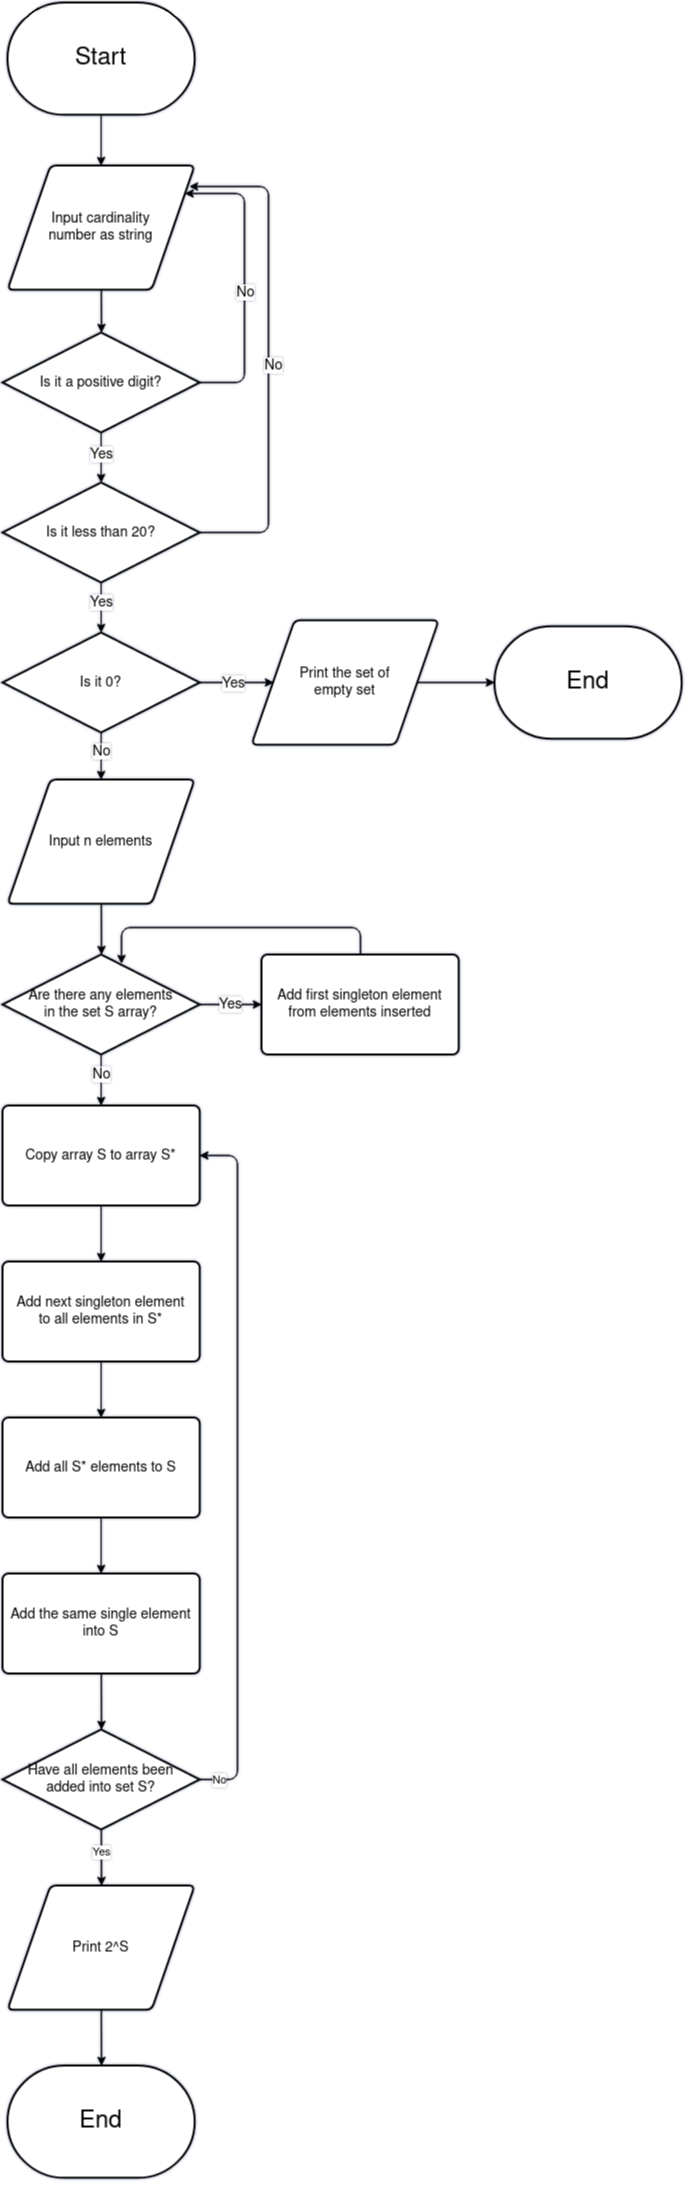
\includegraphics[width=0.45\textwidth]{figures/cs.png}
	\caption{Flowchart of the implemented algorithm}
	\label{fig:algorithm}
\end{figure}
\newpage
\section{Problem 2}
\subsection{Important Remarks and Explanations}
\begin{itemize}
	\item Note that for the ease of use the input of directory and name of file were separated. This will allow the user to have a singular working directory with multiple files without having to specify the directory for the file each time.
	\item Every scanf function implemented has been considered to avoid overflow. For example, in the code below we take input of $127$ :
		\begin{lstlisting}[language = C , caption={scanf overflow protection} , frame = trBL , firstnumber = last , escapeinside={(*@}{@*)}]
		...
		char file[128];
		scanf("%127s", file);
		...
		\end{lstlisting}
	\item For insertion of line, pasting a line etc. it was decided to be written by writing a temporary file with the new line and then replacing the old file with the temp file. The main advantage of using this method over appending the current one is that if the program abruptly shuts down in the middle of writing, then it does not edit the original file and keeps it as is. i.e., 
		\begin{lstlisting}[language = C , caption={Temporary file} , frame = trBL , firstnumber = last , escapeinside={(*@}{@*)}]
		...
					// Combine input directory and input file for writing

			strcpy(tempDirectoryAndFile, directory);
			strcat(tempDirectoryAndFile, "/");
			strcat(tempDirectoryAndFile, ".temp");

			strcat(insertLine, "\n");

			FILE *fp;
			FILE *temp;
			fp = fopen(directoryAndFile, "r");

			temp = fopen(".temp", "w");
			temp = fopen(tempDirectoryAndFile, "w");
			
			while((c = fgetc(fp)) != EOF) { /* copy the text for all lines in temp except the selected line, where the selected line has selected text inserted to it */
				if (c == '\n') {
					lineCounter++;
				}
				if (lineCounter != lineNumber) {
					fputc(c, temp);
				}
				else {
					fputs("\n", temp); /* to ensure correct spacing */
					fputs(insertLine, temp);
					lineCounter++;
				}
			}
		...
		\end{lstlisting}
	\item Appropriate array sizes were chosen with the consideration that they are big enough to what the user would require for everyday use.
	\item It was chosen to add the symbol $\backslash$ between the name of file and the parent working directory input as by definition it lacks the symbol $\backslash$, i.e. the method
		\begin{lstlisting}[language = C , caption={Concatenation of directory and name} , frame = trBL , firstnumber = last , escapeinside={(*@}{@*)}]
		...
			void getLocation() {
				strcpy(directoryAndFile, directory);
				strcat(directoryAndFile, "/");
				strcat(directoryAndFile, file);
			}
		...
		\end{lstlisting}

	\item All commands have appropriate error checking. That is, we ensure that commands that require the correct input e.g. appendl have the file and directory selected correctly. Some examples include:
		\begin{lstlisting}[language = C , caption={String integer method} , frame = trBL , firstnumber = last , escapeinside={(*@}{@*)}]
		...
		short integerCheck(char s[]) {
			for(unsigned int i = 0; s[i] != '\0'; i++) {
			if (isdigit(s[i]) == 0)
				return 0;
			}
		return 1;
		}	
		...
		\end{lstlisting}
		\begin{lstlisting}[language = C , caption={Acceptable number in file method} , frame = trBL , firstnumber = last , escapeinside={(*@}{@*)}]
	...	
	unsigned int lineNumberCheck(unsigned int k, char n[]) {
		if (integerCheck(n) == 1) { /* check if inputted data is an integer number */
			char *ptr;
			k = strtoul(n, &ptr, 10);

			unsigned int lineCounter = 0; 
			char c; 
			FILE *fp; 
			fp = fopen(directoryAndFile, "r"); 

			while((c = fgetc(fp)) != EOF) {
				if (c == '\n') { /* check if character is a new line, and +1 counter if so */
					lineCounter++;
				}
			}

			if (k <= lineCounter) { /* check if our number can be used for the operation as it we can only do it on range of numbers that are present in the file */
				fixedLine = 1;
				return k;
			} else {
				printf("Your selected line number is too big.\n");
				fixedLine = 0;
			}
		} else {
			printf("Your selected line number is not an acceptable number.\n");
			fixedLine = 0;
		}
	
	}
	...
		\end{lstlisting}
		\begin{lstlisting}[language = C , caption={fopen Error Check} , frame = trBL , firstnumber = last , escapeinside={(*@}{@*)}]
		if (fp == NULL) {
    			perror("Failed to open file: ");
    			printf("\n The program will exit.\n");
    			exit(1);
		}
		\end{lstlisting}
		\begin{lstlisting}[language = C , caption={Location Error Check} , frame = trBL , firstnumber = last , escapeinside={(*@}{@*)}]
	...		
	void validLocation() {
			DIR* tempDirectoryAndFile = opendir(directoryAndFile);
			DIR* tempDirectory = opendir(directory);

			if (tempDirectory) {
				fixedDir = 1; /* Value used to break loop */
			} else {
				fixedDir = 0;  /* Value used to repeat loop */
			}
			if (tempDirectoryAndFile) {
				printf("The path %s has been selected successfully.\n", directoryAndFile); /* Check if path depending on current inputs WITHOUT file input exists */
				fixed = 0; /* Value used to repeat loop */
				closedir(tempDirectoryAndFile);
			} else if (ENOENT == errno) {
				printf("The path %s does not exist.\n", directoryAndFile); /* Check if error because it does not exist */
				fixed = 0; /* Value used to repeat loop */
			} else if (ENOTDIR == errno && tempDirectory) {
				printf("The path %s has been selected successfully. \n", directoryAndFile); /* Check if path depending on current inputs exists and would be a valid directory without the existence of file */
				fixed = 1; /* Value used to break loop */
			} else {
				printf("The path %s could not be opened.\n", directoryAndFile); /* Other errors */
				fixed = 0; /* Value used to repeat loop */
			}
	}
	...
		\end{lstlisting}
	\item It was decided that the log will contain only logs of commands that write or change the file at any point. Thus, commands that read are not recorded, as it does not change anything.
	\item A help function was added to help the user navigate and use the software.
	\item Unsigned integer was used as the preferred way to represent numbers because things such as line number cannot be negative.
	\item The design decision to always ask for input was done because its ease of usability. That is, even if a person types something wrong, it redirects them to help. Furthermore, because there are a lot of functions that can be used together after each other, it would also make sense to constantly ask for input.
	i.e.,
	\begin{lstlisting}[language = C , caption={Constant input} , frame = trBL , firstnumber = last , escapeinside={(*@}{@*)}]
	...
		while (1) {
			char command[20];	

			scanf("%19s", command); /* command input */
		...
	\end{lstlisting}
	\begin{lstlisting}[language = C , caption={Help message trigger and command} , frame = trBL , firstnumber = last , escapeinside={(*@}{@*)}]
...
		if (strcmp(command, "help") != 0 && strcmp(command, "dirf") != 0 && strcmp(command, "namef") != 0 && strcmp(command, "copyl") != 0 && strcmp(command, "pastel") != 0 && strcmp(command, "log") != 0 && strcmp(command, "exit") != 0 && strcmp(command, "deletef") != 0 && strcmp(command, "readf") != 0 && strcmp(command, "copyf") != 0 && strcmp(command, "createf") != 0 && strcmp(command, "linef") != 0 && strcmp(command, "deletel") != 0 && strcmp(command, "showl") != 0 && strcmp(command, "insertl") != 0 && strcmp(command, "appendl") != 0) {
			printf("Unknown command. Type <help> for a list of commands.\n");
		}

		// Help command that prints existing commands

		if (strcmp(command, "help") == 0) {
			printf("=============FILE SELECTION=============\n");
			printf("Change parent directory:\n");
			printf("dirf\n");
			printf("Change file:\n");
			printf("namef\n");
			printf("=============FILE MANAGEMENT=============\n");
			printf("Delete selected file:\n");
			printf("deletef\n");
			printf("Read selected file:\n");
			printf("readf\n");
			printf("Copy selected file:\n");
			printf("copyf\n");
			printf("Create file:\n");
			printf("createf\n");
			printf("=============LINE MANAGEMENT=============\n");
			printf("Number of lines in file:\n");
			printf("linef\n");
			printf("Append a line:\n");
			printf("appendl\n");
			printf("Insert a line:\n");
			printf("insertl\n");
			printf("Show a line:\n");
			printf("showl\n");
			printf("Delete a line:\n");
			printf("deletel\n");
			printf("Copy a line:\n");
			printf("copyl\n");
			printf("Paste copied line: \n");
			printf("pastel\n");
			printf("=============OTHER=============\n");
			printf("Exit the program:\n");
			printf("exit\n");
			printf("View writing log:\n");
			printf("log\n");
			}
		...
	\end{lstlisting}
	\item It was decided to take directory and name of file separately as it makes switching between a working directory very easy. Having to ask directory every time would make it tedious for the user.
	\item It was decided that the location of the log will always be placed in the same directory as the file editor for ease of access
	\item The command names, as it is convenient for them to be a singular word in the perspective of the software engineer, were designed by adding "l" or "f" to the end of the name of function, which represents line and file respectively.
	\item To avoid repeated code, methods were added, e.g. number of lines before in log, after etc.
	\item If a file could not be opened i.e. $==\text{NULL}$, then it was decided that the program will exit. This is because the amount of errors that could cause this condition are tremendous. As such, the error message is printed before for the user to check and fix if possible. Indeed, a precaution was taken to avoid this error by ensuring that the directory entered is existing, which would be a very common cause of issue.
\end{itemize}
\subsection{Explanation of commands}
\subsubsection{Explanation of all Operations}
\- \- \- \- \- \- 
\textbf{dirf} \\
Function: change the parent working directory.\\
Description: works by storing the input parent working directory as a string. Concatenates the input string with namef input string. Then checks if the combined string exists. \\
Code:
\begin{lstlisting}[language = C , caption={dirf} , frame = trBL , firstnumber = last , escapeinside={(*@}{@*)}]
		if (strcmp(command, "dirf") == 0) {
			printf("Please type the parent directory that you want to open:\n");
			scanf("%255s", directory);
			getLocation(); /* combines dirf and namef */
			validLocation(); /* checks if combination of dirf and namef is valid */
		}
\end{lstlisting}

\textbf{namef}\\
Function: change the name of the working file. \\
Description: works by storing the input name as a string. Concatenates the input string with dirf input string. Then checks if the combined string exists.\\
Code:
\begin{lstlisting}[language = C , caption={namef} , frame = trBL , firstnumber = last , escapeinside={(*@}{@*)}]
		if (strcmp(command, "namef") == 0) {
			printf("Please type the full name of file that you want to edit:\n");
		       	scanf("%127s", file);
			getLocation(); /* combines dirf and namef */
			validLocation(); /* checks if combination of dirf and namef is valid */
		}
\end{lstlisting}

\textbf{deletef}\\
Function: deletes the selected file.\\
Description: checks if the selected file exists. If not, forces the user to select until it does. Once existence has been confirmed, it deletes the file and logs the operation.\\ 
Code: 
\begin{lstlisting}[language = C , caption={deletef} , frame = trBL , firstnumber = last , escapeinside={(*@}{@*)}]
		if (strcmp(command, "deletef") == 0) {
			forceFixLocation(); /* required correct file input */
			if (remove(directoryAndFile) == 0) {
				printf("File has been deleted successfully.\n");
			} else {
				printf("Error. File could not be deleted. \n");
			}
			standardLogMessage("deletef"); /* write it to log */
		}
\end{lstlisting}

\textbf{readf}\\
Function: prints out all characters in the selected file to terminal. \\
Description: checks if the selected file exists. If not, forces the user to select until it does. Opens the file in read mode, and reads each character until end of line of file. Prints out each read character into terminal. Closes the file. \\
\begin{lstlisting}[language = C , caption={readf} , frame = trBL , firstnumber = last , escapeinside={(*@}{@*)}]
		if (strcmp(command, "readf") == 0) {
			forceFixLocation(); /* required correct file input */
			FILE *fp; 
			char c; 
   			fp = fopen (directoryAndFile, "r");
			
			// Check if file opened correctly

			if (fp == NULL) {
    			perror("Failed to open file: ");
    			printf("\n The program will exit.\n");
    			exit(1);
			}

			while((c = fgetc(fp)) != EOF) {
				printf("%c", c); /* print characters found in file until end of file */
			}
			printf("\n");
			fclose(fp);
		}
\end{lstlisting}

\textbf{copyf} \\
Function: copies the selected file into another directory chosen by the user. \\
Description: checks if the selected file exists. If not, forces the user to select until it does. Asks user input for the directory they wish to copy to until the directory exists. Having the same directory is not allowed, and thus is an exception to accepted directories as well. Once directory has been validated, opens the selected file in read mode and writes the new file in the selected directory. Copies each character in the new file until end of line. Logs the operation. Closes both files. \\
Code:
\begin{lstlisting}[language = C , caption={copyf} , frame = trBL , firstnumber = last , escapeinside={(*@}{@*)}]
		...
		if (strcmp(command, "copyf") == 0) {
			forceFixLocation(); /* required correct file input */
			int newLocation = 0;
			char c;
			char copyDirectory[256];
			char copyDirectoryAndFile[385];

			// Similar to validLocation and forceFixLocation, forced correct input is required for the target copy directory.

			while (newLocation == 0) {
				printf("Please enter the parent directory of the new file:\n");
				scanf("%127s", copyDirectory);

				// Combine input directory and file name for writing

				strcpy(copyDirectoryAndFile, copyDirectory);
				strcat(copyDirectoryAndFile, "/");
				strcat(copyDirectoryAndFile, file);

				// Check if the directory exists

				DIR* createTempDirectoryAndFile = opendir(copyDirectoryAndFile);
				DIR* createTempDirectory = opendir(copyDirectory);
			
				if ((createTempDirectory) && strcmp(copyDirectory, directory) != 0) {
					printf("The path %s has been selected successfully.\n", copyDirectory);
					closedir(createTempDirectory);
					newLocation = 1; /* If selected successfully, we break out of the loop */
				} else if (ENOENT == errno) {
					printf("The path %s does not exist.\n", copyDirectoryAndFile);
				} else {
					printf("The path %s could not be opened.\n", copyDirectory);
				}
			}

				FILE *fp;
				FILE *copy;

				fp = fopen(directoryAndFile, "r");
				copy = fopen(copyDirectoryAndFile, "w");

				// Check if file opened correctly

				if (fp == NULL) {
    			perror("Failed to open file: ");
    			printf("\n The program will exit.\n");
    			exit(1);
				}
			
				while((c = fgetc(fp)) != EOF) {
					fputc(c, copy); /* write characters found in file until end of file */
				}

				fclose(fp);
				fclose(copy);

				// Log specialiesd for this particular operation

				standardLogMessage("copyf");
				FILE *log;
				log = fopen("log.txt", "a");
				fputs("Copied to the path ", log);
				fputs(copyDirectory, log);
				fputs(". \n", log);

		}
		...
\end{lstlisting}

\textbf{createf}\\
Function: creates a new file in the currently selected working directory with an input name. \\
Description: checks if the selected working directory is valid, if not, keep asking until it is valid. Gets input from user for name of file. Creates the file by opening with write mode. Closes the file. Logs the operation. \\
Code:
\begin{lstlisting}[language = C , caption={createf} , frame = trBL , firstnumber = last , escapeinside={(*@}{@*)}]
	...
		if (strcmp(command, "createf") == 0) {

			// Similar to validLocation and forceFixLocation, designed for the new input within the method for the target location instead

			while(fixedDir == 0) {
				printf("The path %s has could not be selected. Please enter a new parent directory:\n", directory);
				scanf("%255s", directory);
				getLocation(); /* Combine it to get full location */
				validLocation(); /* Check if it is a valid location that breaks the loop*/
			}

			char createFile[128];
			char createDirectoryAndFile[385];

			printf("Please enter the name of the new file:\n");
			scanf("%255s", createFile);

			// File location

			strcpy(createDirectoryAndFile, directory);
			strcat(createDirectoryAndFile, "/");
			strcat(createDirectoryAndFile, createFile)

			FILE *fp; 
			fp = fopen (createDirectoryAndFile, "w"); 
			fclose(fp);

			// Log specialised for this particular operation

			FILE *log;
			log = fopen("log.txt", "a");
			fputs("The operation ", log);
			fputs("createf", log);
			fputs(" was commenced in the path ", log);
			fputs(createDirectoryAndFile, log);
			fputs(". \n", log);
			fclose(log);

			printf("%s has been written successfully.\n", createDirectoryAndFile);
		}
	...
\end{lstlisting}

\textbf{linef} \\
Function: wounts the number of lines in the selected file. \\
Description: checks if the selected file exists. If not, forces the user to select until it does. Reads all characters until end of file and increments if it finds the character '$\backslash $n'. Once found, increment. Prints this number. \\
\begin{lstlisting}[language = C , caption={linef} , frame = trBL , firstnumber = last , escapeinside={(*@}{@*)}]
		if (strcmp(command, "linef") == 0) {
			forceFixLocation(); /* required correct file input */
			unsigned int lineCounter = 0; 
			char c; 
			FILE *fp; 
			fp = fopen(directoryAndFile, "r"); 

			// Check if file opened correctly

			if (fp == NULL) {
    			perror("Failed to open file: ");
				printf("\n The program will exit.\n");
    			exit(1);
			}

			while((c = fgetc(fp)) != EOF) {
				if (c == '\n') { /* check if character is a new line, and +1 counter if so */
					lineCounter++;
				}
			}
			printf("There are %u lines in the path %s. \n", lineCounter, directoryAndFile);
		}
\end{lstlisting}

\textbf{appendl} \\
Function: write a new line at the end of the file. \\
Description: checks if the selected file exists. If not, forces the user to select until it does. Logs the number of lines. Opens the file in append mode. Asks for input line and adds it to file. Logs the operation. Closes the folder and logs the number of lines again. \\
Code:
\begin{lstlisting}[language = C , caption={appendl} , frame = trBL , firstnumber = last , escapeinside={(*@}{@*)}]
		if (strcmp(command, "appendl") == 0) {
			forceFixLocation(); /* required correct file input */
			lineLogBefore(); /* log amount of lines in file */
			char insertLine[512];
			FILE *fp;
			fp = fopen(directoryAndFile, "a"); 

			// Check if file opened correctly

			if (fp == NULL) {
    				perror("Failed to open file: ");
    				printf("\n The program will exit.\n");
    				exit(1);
			}

			printf("Please type the line text that you wish to insert:\n");
			scanf(" %519[^\n]s", insertLine);
			printf("The line %s was appended successfully in the path %s.", insertLine, directoryAndFile);

			standardLogMessage("appendl"); /* write it to log */

			// Ensuring correct spacing in the file

			strcat(insertLine, "\n");
			fputs(insertLine, fp);

			fclose(fp);

			lineLogAfter(); /* log amount of lines in file */
		}
\end{lstlisting}

\textbf{insertl} \\
Function: inserts a line of text to a desired line number. \\
Description: checks if the selected file exists. If not, force the user to select until it does.  Logs the number of lines. Gets input for line number and line that requires to be inserted. Inserts the line by creating a duplicate of the file (called .temp) with the inserted line. Then, deletes the original file and replaces it by the temporary file. Logs the operation. Closes the opened folders and logs the number of lines. \\
Code:
\begin{lstlisting}[language = C , caption={insertl} , frame = trBL , firstnumber = last , escapeinside={(*@}{@*)}]
		if (strcmp(command, "insertl") == 0) {
			forceFixLocation(); /* required correct file input */
			unsigned int lineNumber;
			unsigned int lineCounter = 1;
			char tempDirectoryAndFile[262];
			char number[10];
			char insertLine[512];
			char c;
			lineLogBefore();

			// Enter line number and check for errors

			while(fixedLine == 0){
				printf("Please enter the line number that you wish to insert to:\n");
				scanf("%s", number);
				lineNumberCheck(lineNumber, number);
			}

			selectedLineLog(lineNumber);
			printf("Please the line text that you wish to insert: \n");
			scanf(" %519[^\n]s", insertLine);

			// Combine input directory and input file for writing

			strcpy(tempDirectoryAndFile, directory);
			strcat(tempDirectoryAndFile, "/");
			strcat(tempDirectoryAndFile, ".temp");

			strcat(insertLine, "\n");

			FILE *fp;
			FILE *temp;
			fp = fopen(directoryAndFile, "r");

			// Check if file opened correctly

			if (fp == NULL) {
    			perror("Failed to open file: ");
				printf("\n The program will exit.\n");
    			exit(1);
			}

			temp = fopen(".temp", "w");
			temp = fopen(tempDirectoryAndFile, "w");
			
			while((c = fgetc(fp)) != EOF) { /* copy the text for all lines in temp except the selected line, where the selected line has selected text inserted to it */
				if (c == '\n') {
					lineCounter++;
				}
				if (lineCounter != lineNumber) {
					fputc(c, temp);
				}
				else {
					fputs("\n", temp); /* to ensure correct spacing */
					fputs(insertLine, temp);
					lineCounter++;
				}
			}
\end{lstlisting}

\textbf{showl} \\
Function: prints the content of a particular line to terminal. \\
Description: checks if the selected file exists. If not, force the user to select until it does. Asks for line number and then opens the file. Begins to read all characters, increments line counting number and then when it reaches the specified line, prints the characters out. \\
Code:
\begin{lstlisting}[language = C , caption={showl} , frame = trBL , firstnumber = last , escapeinside={(*@}{@*)}]
		if(strcmp(command, "showl") == 0) {
			forceFixLocation(); /* required correct file input */
			unsigned int lineNumber;
			char number[10];

			// Enter line number and check for errors

			while(fixedLine == 0){
				printf("Please enter the line number that you wish to insert to:\n");
				scanf("%s", number);
				lineNumberCheck(lineNumber, number);
			}

			char c;
			unsigned int lineCounter = 1;
			FILE *fp;
			fp = fopen(directoryAndFile, "r");

			// Check if file opened correctly

			if (fp == NULL) {
    			perror("Failed to open file: ");
    			printf("\n The program will exit.\n");
    			exit(1);
			}

			while((c = fgetc(fp)) != EOF) {
				if (c == '\n') {
					lineCounter++;
				}

				if (lineCounter == lineNumber) {
					printf("%c", c); /* print that character until end of file */
				}
			}
			printf("\n");
		}
\end{lstlisting}

\textbf{deletel} \\
Function: deletes a specified line in the file. \\
Description: checks if the selected file exists. If not, force the user to select until it does. Logs the number of lines. Takes input for the line number. Creates a temporary folder where it copies every line but skips the selected line. Deletes the original folder and replaces it with the temporary folder. Closes the opened files. Logs the amount of lines. \\
Code: 
\begin{lstlisting}[language = C , caption={deletel} , frame = trBL , firstnumber = last , escapeinside={(*@}{@*)}]
		if (strcmp(command, "deletel") == 0) {
			forceFixLocation(); /* required correct file input */

			lineLogBefore(); /* log amount of lines in file */

			unsigned int lineNumber;
			unsigned int lineCounter = 1;
			char tempDirectoryAndFile[262];
			char number[10];
			char c;

			// Enter line number and check for errors

			while(fixedLine == 0){
				printf("Please enter the line number that you wish to delete:\n");
				scanf("%s", number);
				lineNumber = lineNumberCheck(lineNumber, number);
			}

			// Combine inpput directory and input file for writing

			strcpy(tempDirectoryAndFile, directory);
			strcat(tempDirectoryAndFile, "/");
			strcat(tempDirectoryAndFile, ".temp");

			FILE *fp;
			FILE *temp;
			fp = fopen(directoryAndFile, "r");

			// Check if file opened correctly

			if (fp == NULL) {
    			perror("Failed to open file: ");
    			printf("\n The program will exit.\n");
    			exit(1);
			}
			
			temp = fopen(tempDirectoryAndFile, "w");

			while((c = fgetc(fp)) != EOF) {
				if (c == '\n') {
					lineCounter++;
				}
				if (lineCounter != lineNumber) {
					fputc(c, temp);
				}
			}

			printf("Line %u was deleted successfully in the path %s. \n", lineNumber, directoryAndFile);
			standardLogMessage("deletel"); /* write it to log */

			// Replace selected file with temp

			fclose(fp);
			remove(directoryAndFile);
			fclose(temp);
			rename(tempDirectoryAndFile, directoryAndFile);

			lineLogAfter(); /* log amount of lines in file */
		}
\end{lstlisting}

\textbf{copyl} \\
Function: copies a specified line to memory. \\
Description: checks if the selected file exists. If not, force the user to select until it does. Takes input for the line number. Opens the file and gets the content in the inserted line number.Closes the file.
Code:
\begin{lstlisting}[language = C , caption={copyl} , frame = trBL , firstnumber = last , escapeinside={(*@}{@*)}]
		if (strcmp(command, "copyl") == 0) {
			forceFixLocation(); /* required correct file input */
			unsigned int lineCounter = 0;
			unsigned int lineNumber;
			char number[10];

			// Enter line number and check for errors

			while(fixedLine == 0){
				printf("Please enter the line number that you wish to insert to:\n");
				scanf("%s", number);
				lineNumberCheck(lineNumber, number);
			}

			FILE *fp;
			fp = fopen(directoryAndFile, "r");

			while(fgets(lineCopy, 511, fp) != NULL) {
				if (lineCounter == lineNumber) { /* find the selected line and store it into a string */
					fclose(fp);
					break;
				} else {
					lineCounter++;
				}

			}
			printf("The line %s was copied successfully in the path %s. \n", lineCopy, directoryAndFile);
			fclose(fp);
		}
\end{lstlisting}

\textbf{pastel} \\
Function: pastes the copied string. \\
Description: checks if the selected line exists. If not, force the user to select until it does. Takes input for the line number. Logs the line numbers. Opens the file and creates a temporary file. Copies the file with the exception of the selected line, where the selected line has the copied content. Logs the operation. Closes the folders. \\
Code: 
\begin{lstlisting}[language = C , caption={pastel} , frame = trBL , firstnumber = last , escapeinside={(*@}{@*)}]
		if (strcmp(command, "pastel") == 0) {
			forceFixLocation(); /* required correct file input */
			unsigned int lineNumber;
			char number[10];

			// Enter line number and check for errors

			while(fixedLine == 0){
				printf("Please enter the line number that you wish to insert to:\n");
				scanf("%s", number);
				lineNumberCheck(lineNumber, number);
			}

			lineLogBefore();  /* log amount of lines in file */
			selectedLineLog(lineNumber); /* log line  number*/

			unsigned int lineCounter = 1;
			char tempDirectoryAndFile[262];
			char c;
			FILE *fp;
			FILE *temp;
			fp = fopen(directoryAndFile, "r");

			// Combine input directory and input file for writing

			strcpy(tempDirectoryAndFile, directory);
			strcat(tempDirectoryAndFile, "/");
			strcat(tempDirectoryAndFile, ".temp");

			// Check if file opened correctly

			if (fp == NULL) {
    			perror("Failed to open file: ");
				printf("\n The program will exit.\n");
    			exit(1);
			}

			temp = fopen(".temp", "w");
			temp = fopen(tempDirectoryAndFile, "w");
			
			while((c = fgetc(fp)) != EOF) { /* copy the text for all lines in temp except the selected line, where the selecteed line has selected text inserted to it */
				if (c == '\n') {
					lineCounter++;
				}
				if (lineCounter != lineNumber) {
					fputc(c, temp);
				}
				else {
					fputs("\n", temp);
					fputs(lineCopy, temp);
					lineCounter++;
				}
			}

			printf("The line %s was pasted successfully in the path %s.", lineCopy, directoryAndFile);

			standardLogMessage("pastel");

			// Replace selected file with temp

			fclose(fp);
			remove(directoryAndFile);
			fclose(temp);
			rename(tempDirectoryAndFile, directoryAndFile);

			lineLogAfter(); /* log amount of lines in file */
		}
\end{lstlisting}

\textbf{exit} \\
Function: exits the program. \\
Description: logs the exit and exits the program. \\
Code:
\begin{lstlisting}[language = C , caption={exit} , frame = trBL , firstnumber = last , escapeinside={(*@}{@*)}]
		if (strcmp(command, "exit") == 0) {
			FILE *log;
			log = fopen("log.txt", "a");
			fputs("Program closed using exit \n", log);
			fclose(log);
			exit(0);
		}
\end{lstlisting}

\textbf{log} \\
Function: reads log.txt \\
Description: opens log.txt and prints out all characters found in log.txt until end of file. Closes the file.
Code:
\begin{lstlisting}[language = C , caption={log} , frame = trBL , firstnumber = last , escapeinside={(*@}{@*)}]
		if (strcmp(command, "log") == 0) {
			FILE *fp; 
			char c;
   			fp = fopen ("log.txt", "r");
			while((c = fgetc(fp)) != EOF) {
				printf("%c", c); 
			}
			printf("\n");
			fclose(fp);
		}
\end{lstlisting}
\subsubsection{Use of Newly Implemented Operations}
Two new operations were added. These operations are the following:
\begin{itemize}
	\item Choose directory
	\item Copy and paste a line	
\end{itemize}
\textbf{Choosing Directory - dirf}
\begin{flushleft}
	Being able to choose a directory is a powerful tool for the user. It greatly extends the usability of the software that was written. This way the user would not be required to move the compiled file to the folder that they want to edit. The whole program was designed with changing directory in mind, therefore all implemented commands can utilise this new operation. It greatly saves time for the user and more importantly the amount of external operations they would have to do e.g. cut/copy the compiled file into another folder, open it etc.
\end{flushleft}
\textbf{Copy and paste a line - copyl and pastel}
\begin{flushleft}
With the implementation of choosing directory, it would also make sense if we had the ability to copy and then paste a line into anywhere desired. Our first new operation greatly extends the usability of this function, that is, the two synchronise very well. Not only we are allowed to copy a line and paste it into the same file, but we also gain the ability to paste the line into any other file that we can choose to edit. Furthermore, the person can easily make this a 'cut' operation by using remove. This way, if the user is required to, for example, move code from one file to another to reuse it, this operation makes it possible without having to remember it. 
\end{flushleft}
\subsection{Log}
The implementation of log included the appending of log.txt which is located in the same directory as the C program. The idea is that the log pinpoints where edits happened, not pinpointing the exact changed content. This means that the log was designed to record lines which were edited, and records only edits. In particular, the following generic message code was added as a method to use:
\begin{lstlisting}[language = C , caption={Standard log message} , frame = trBL , firstnumber = last , escapeinside={(*@}{@*)}]
	void standardLogMessage(char o[]) {
		FILE *log;
		log = fopen("log.txt", "a");
		fputs("The operation ", log);
		fputs(o, log);
		fputs(" was commenced in the path ", log);
		fputs(directoryAndFile, log);
		fputs(". \n", log);
		fclose(log);
	}
\end{lstlisting}
And as per request, places where line change strictly happens, the following methods were added to record before and after number of lines respectively:
\begin{lstlisting}[language = C , caption={Number of lines before} , frame = trBL , firstnumber = last , escapeinside={(*@}{@*)}]
	void lineLogBefore() {
		unsigned int lineCounter = 0; 
		char c; 
		char lineNumber[10];
		FILE *fp; 
		FILE *log;
		log = fopen("log.txt", "a"); 
		fp = fopen(directoryAndFile, "r"); 
		while((c = fgetc(fp)) != EOF) {
			if (c == '\n') { /* check if character is a new line, and +1 counter if so */
				lineCounter++;	
			}
		}
		fclose(fp);
		sprintf(lineNumber, "%u", lineCounter);
		fputs("Before operation, there are ", log);
		fputs(lineNumber, log);
		fputs(" lines in the path ", log);
		fputs(directoryAndFile, log);
		fputs(". \n", log);
		fclose(log);
	}
\end{lstlisting}
\begin{lstlisting}[language = C , caption={Number of lines after } , frame = trBL , firstnumber = last , escapeinside={(*@}{@*)}]
	void lineLogAfter() {
		unsigned int lineCounter = 0; 
		char c; 
		char lineNumber[10];
		FILE *fp; 
		FILE *log;
		log = fopen("log.txt", "a");
		fp = fopen(directoryAndFile, "r"); 
		while((c = fgetc(fp)) != EOF) {
			if (c == '\n') { /* check if character is a new line, and +1 counter if so */
				lineCounter++;
			}
		}
		fclose(fp);
		sprintf(lineNumber, "%u", lineCounter);
		fputs("After operation, there are ", log);
		fputs(lineNumber, log);
		fputs(" lines in the path ", log);
		fputs(directoryAndFile, log);
		fputs(". \n", log);
		fputs("================================================================================ \n", log); /* Line seperator to make log easier to read */
		fclose(log);
	}
\end{lstlisting}
And indeed, a method to record which line was selected for a particular editing operation:
\begin{lstlisting}[language = C , caption={selectedLineLog} , frame = trBL , firstnumber = last , escapeinside={(*@}{@*)}]
	void selectedLineLog(unsigned int i) {
		char selectedLineNumber[10];
		FILE *log;
		log = fopen("log.txt", "a");
		sprintf(selectedLineNumber, "%u", i);
		fputs("Line ", log);
		fputs(selectedLineNumber, log);
		fputs(" was selected. \n", log);
		fclose(log);
	}
\end{lstlisting}
\nocite{*}
\newpage
\bibliographystyle{apacite}
\bibliography{bibliography}
\end{document}
